\documentclass[journal,onecolumn]{IEEEtran} % with page numbers
\usepackage{xcolor}
\usepackage{booktabs, multirow}
\usepackage{tabularx}
\usepackage{ragged2e}
\usepackage{graphicx}
\usepackage{subfigure}
\usepackage{amsmath}
\usepackage{underscore}
\usepackage{caption}
\usepackage{multirow}
\usepackage{cite}
\usepackage{fancyhdr}

\sloppy

\captionsetup[table]{position=bottom} 
\renewcommand{\arraystretch}{1.5}

\renewcommand\thesection{\arabic{section}}
\renewcommand\thesubsection{\thesection.\arabic{subsection}}
\renewcommand\thesubsubsection{\thesubsection.\arabic{subsubsection}}

\renewcommand\thesectiondis{\arabic{section}}
\renewcommand\thesubsectiondis{\thesectiondis.\arabic{subsection}}

\makeatletter %needed
	\renewcommand{\@seccntformat}[1]
	{{\csname the#1\endcsname\hspace{0.5em}}}
\makeatother

\pagestyle{fancy}
\fancyhf{}
\renewcommand{\headrulewidth}{0pt}
\cfoot{\thepage}

\begin{document}

\title{\LARGE Preparation phase report: A digital twin of a microbrewery---a case study investigating DT model integration and orchestration techniques}
\author{\IEEEauthorblockN{Ander Lee \\
	\texttt{a.lee@student.tue.nl} \\
	Version 2.3.0 \\
	April 2022} \\}
\maketitle

\tableofcontents
\pagebreak

\section{Introduction}
The digital twin (DT) model was first introduced by Grieves in a 2002 presentation \cite{Grieves2019}. At the time it was referred to as a concept for Product Lifecycle Management (PLM). The model asserts that systems are dual in nature, that is, a system has a physical twin and a virtual twin. The premise of the model is that the two sides are bound together via a data link. This link is bidirectional that it transfers data from the physical space to update the virtual space, and vice versa. 

The association to PLM implies that a DT is a dynamic model that adapts to specific stages in the product's lifecycle. The stage changes made in either space are promptly translated to the subsequent outcomes in the other space. An example in practice could be, an operator---a real human or an autonomous decision making program---makes a design tuning to the virtual mock-up, this change consequently modifies the behaviors of the manufactured physical product. The physical product which possesses the latest information received from the virtual space, is deployed and operates in the intended context. From then the physical product collects data about the system itself or the reactions arising from its interactions with the environment and sends them back to the virtual space. These behavioral characteristics of DTs make a great distinction from simulations, which are commonly confused with DTs. To simply put it, we consider that DTs take a step further by using simulations to influence physical space. This idea is particularly helpful to the products with very broad scale lifecycle, both in terms of timeline and complexity. As we can see soon this is a reason why DTs have gained successe in many industries.

After Grieves' proposal of using DTs for PLM, the early adopters of this concept were aerospace engineering organizations such as NASA and US Air Force \cite{Grieves2019}. It is not difficult to realize this is more than just a coincidence. The lifecycle of aircraft is broad, on average, between 20 to 35 years \cite{boeing}.The design phase alone can already take many years, much less the operation and maintenance phase, which can last up to several decades. Even if narrowed to just a snapshot in time, an aircraft is a complex composition of multi-disciplinary outputs. For instance, the jet engine is a high performance mechanical system; the fuel system is largely based on the understandings of chemical reactions; and the communication equipment is the results of electrical and computer designs. Therefore, DTs become one of the best suited methods in this type of circumstance. As time passed, other industries also started to participate in this trend of multi-disciplinary and long-term product lifecycle. Production factories these days use dedicated software to analyze the efficiency of operations and optimize the plant on-the-go \cite{Zheng2018}. Hospitals also use digital assets to aid experiments on drugs and patients \cite{Kwon2022}. As a result, the study of DT development becomes more and more important.

As we have seen the design choices of DT development have grown exponentially in the first two decades of 20th century. In the physical space, this is partially enabled by wireless communication technologies such as remote sensors and cellular networks. On the other hand, in the virtual space more diverse modeling methods are available commercially. A notable progress is shown in big-data models and artificial intelligence models \cite{Duan2019}. Under this premise we start to notice a problem of how to assemble and manage all the available assets together in a DT in order to support the product lifecycle. It is reasonable to assume most tools are not created by the same party, and even if they are, the DT developers will be facing great restrictions due to vendor lock-in. Hence to collaborate using heterogeneous tools we need integration and orchestration. They give attention to aspects as focused as data format merging and unit conversion, to bigger considerations like inter-model scheduling. In this study, we want to investigate what is considered good practice for integration and orchestration. 

As we mentioned before that DTs ultimately aim to support the services in a complex product lifecycle. In this project we also want to verify our findings of integration and orchestration techniques in a case study. We choose a microbrewery as the use case. A brewery has many steps of procedure in order to produce a beer. Among them, a key process that impacts the quality of the beverage is fermentation. The process can be tracked by existing sensors which detect, such as, the alcoholic content and temperatures. Moreover, the conditions of the process are relatively mild, i.e., low temperature, medium high pressure, which allows easy observations. The process is a well studied phenomena, making it easy to construct and evaluate. Therefore, we reckon the construction of microbrewery as a suitable proof-of-concept for DTs. In addition, models for bio-chemical processes often vary significantly in terms of properties and behaviors. Some models might deal with chemical reactions that take place continuously, while other models might deal with discrete observations which only occur periodically. Due to this vast variety, we think it can highlight the integration and orchestration efforts which will be incorporated in our DT services.

In Section \ref{sec:context}, we will describe the growing attention to Industry 4.0 and the role of DTs as part of this trend. After that, the DT domain will be introduced in Section \ref{sec:overview}, in which the term DT will be defined and a reference DT model will be elaborated. Section \ref{sec:sota} examines the current state of the art in DT technologies.

\subsection{Context}\label{sec:context}
As claimed by market analysts \cite{pwc2014} \cite{ibm}, the emerging trend of Industry 4.0 is characterized by widespread digitalization. Hence DTs are becoming more widely adopted as industry moves toward a digital transformation which sets out to improve the transfer of information across the value chain. This will allow stakeholders to share knowledge about the designs, conditions, and logistics of their products and operations through digital artefacts. 

Having a DT, particularly in the manufacturing context, helps to accelerate the design process as it facilitates the use of abundant sensor data and accurate modeling of the physical world to provide deep insights to the engineers. Modeling in DTs has improved significantly in recent years because the concept has evolved from mere simulation to sophisticated mechanisms that can optimize the physical entity based on the data collected. Besides, services in a DT can also offer consistent monitoring of the product throughout its life cycle, allowing optimization of the product’s performance during its lifetime. Other benefits DTs can offer include predictive maintenance and risk assessment. By facilitating the virtual mock-up of the real product, one can overcome the temporal and spatial limitations of experimenting in the physical world, thus greatly reducing the overall cost.

The notion of DT is often associated with the model-driven system engineering (MDSE) paradigm. In MDSE, a complex system is treated holistically. It is described in terms of the interaction between systems, or better known as `system of systems.' The system architecture is represented as models to support requirements, design, analysis and verification activities throughout the lifecycle. The use of modelling helps drive a consistent specification without significantly increasing costs as the system depth extends. Furthermore, DTs aim to capture a comprehensive physical and functional description of the target system. Specifically, virtual entities monitor data from the physical entities, use it to fulfill services which are requested by the user, and may optimize the physical entity. Hence a closed loop of operation is formed. It is found in many studies that DTs have the potential to bring the following benefits \cite{Boschert2016, Macchi2018, Lim2019, Ansari2020, Cai2021, Gurdur2022}:
\begin{itemize}
  \item Reduce maintenance costs during lifecycle.
  \item Reduce errors and inconsistencies across multiple iterations. 
  \item Improve multi-disciplinary collaboration, i.e., engineers from different job functions are able to quickly grasp the high-level overview of the design.
\end{itemize}

These benefits can lead to a more seamless digital transformation in the industry. Hence we argue that further investigations of DT development is regarded important to propel the new wave of industrial transformation. 

\subsection{Domain overview}\label{sec:overview}
This section explains in further detail the concept of DT and its classification. Following that, we describe the challenges of interest for this project.
\subsubsection{Digital twin}\label{sec:dt}
Although the term `digital twin' has been mentioned in much literature, such works seldom share the same definition \cite{Liu2021}. In some works the definition has close resemblance to an integrated simulation, which contains multi-physic, and multi-scale simulations working together \cite{Shafto2012}. However, in some other studies it is defined as a high fidelity digital replica of the physical asset \cite{Schluse2018}. In order to select a suitable definition for the biomanufacturing context, and to keep the later discussions consistent, hereafter we will adopt the classification proposed by Kritzinger et al. \cite{Kritzinger2018}. According to the classification, `digital twin' can be roughly divided in three categories based on the level of data integration between the physical asset and the virtual counterpart:

\begin{figure}[hbt!]
  \centering
  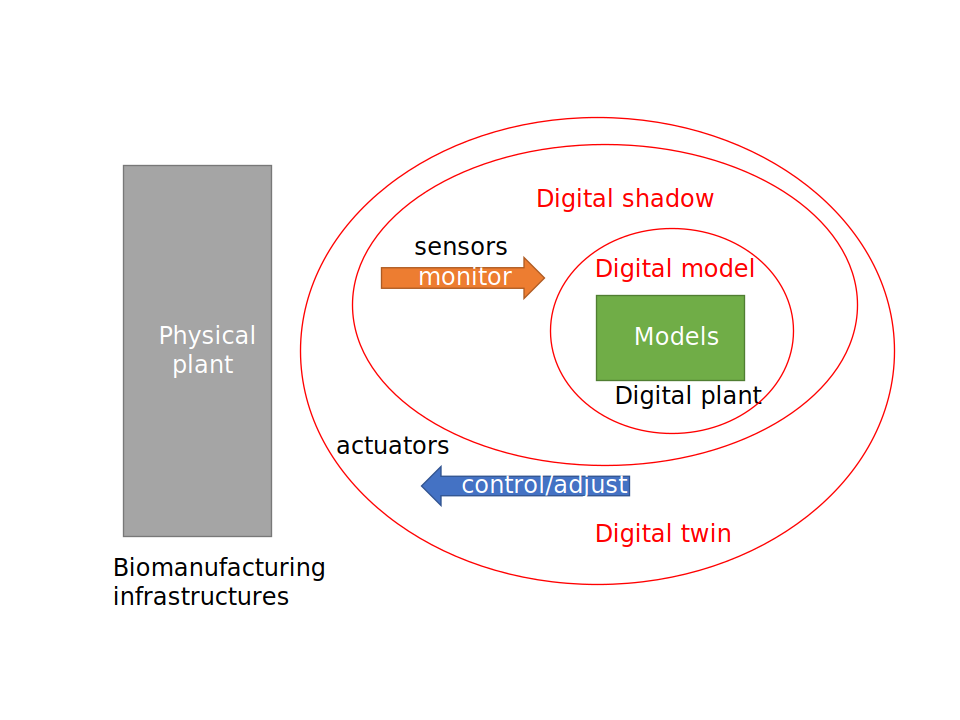
\includegraphics[scale=0.5]{figures/dt.pdf}
  \caption{Classification of digital twin}
  \label{fig:dt}
\end{figure}

\begin{itemize}

  \item \textbf{Digital model}: The virtual object does not involve data exchange with the physical object in an automated fashion. Hence the changes in one part have no direct effect on the other unless updates are performed manually.

  \item \textbf{Digital shadow}: There exists an automated one-way data communication from the physical object to the virtual one.
  
  \item \textbf{Digital twin}: An automation of bi-directional data exchange between the physical object and the virtual object. Changes made in the physical object will be reflected in the virtual object and vice versa. 

\end{itemize}

In a manufacturing plant setting, Data delivered from the physical world to the virtual world is used for monitoring, usually through various types of sensors. The reverse direction---data delivery from the virtual world to the physical world---amounts to adjusting actuators. It is important to note that adjusting or controlling an actuator in a DT denotes a slightly different action than in a traditional control system. In a simple control logic, once a computation produces feedback, the signal will be sent to the actuator to activate certain operations, whereas in a DT, the adjustment data that is sent back to the actuators from the model in the virtual world is meant to calibrate and tune the parameters of an ongoing set of operations. Figure \ref{fig:dt} illustrates the concept of DT that is used throughout this project.

Although Kritzinger's view has an emphasis on a fully automated version of DT, in practice, especially in bio-chemical applications, Udugama et al. \cite{Udugama2020} \cite{Udugama2021} recognize the unskippable need for operator's intervention in many scenarios. Therefore, a more relaxed version of DT can be described, where the digital model automatically generates its results to a human machine interface (HMI) firstly; then the operator will make a decision based on the given data, and update the actuators parameters through the HMI. A similar concept called human-in-the-loop is demonstrated in \cite{Barricelli2020} as part of the design of an athlete DT, where the coach acts as the operator in managing the fitness plan for athletes. Since this project mainly concerns with a microbrewery which is also a biological fermentation process, the relaxed definition of DT is considered relevant.       

\subsubsection{DT model} \label{sec:dtmodel}
The definition in Section \ref{sec:dt} provides a clear view of DTs in term of the data exchange between physical and virtual worlds. A DT model is deemed useful for articulating the management of the interconnections between different parts. Tao et al. \cite{Tao2017} propose a five-dimensional view of DT model as shown in Figure \ref{fig:tao5d}. Each dimension is described as follows:

\begin{figure}[hbt!]
  \centering
  \includegraphics[scale=0.6]{figures/tao5d.pdf}
  \caption{5D view of DT model}
  \label{fig:tao5d}
\end{figure}

\begin{itemize}

  \item \textbf{Physical entity} (PE): A collection of sensors and equipment working collaboratively to collect real-time data for the intended services, meanwhile receiving control orders from the virtual world.    

  \item \textbf{Virtual entity} (VE): A digital mirror, that contains models simulating the physical counterpart with high fidelity. Calibration strategies are generated through comparing the models with entities to support models' evolution.
  
  \item \textbf{Services}: Provides various services to support the management and control of PEs as well as the operation and evolution of VEs. Services are usually requested by the users to fulfill certain functionalities.
       
  \item \textbf{Data}: A shared storage consisting of the raw data from PEs, VEs, and services. It may also be responsible for merging data from various sources to a fused format. 
   
  \item \textbf{Connections}: The connections for all four of the above-mentioned dimensions. Relevant concepts include communication protocols, access ports, etc.
  
\end{itemize}

The 5D view is arguably a helpful reference model to follow when introducing new technological assets toward the incremental development of DTs. Even more generally, it guides stakeholders to quickly survey the basic composition of a DT.

\subsection{Challenges in the domain}\label{sec:challenges}

As DTs become increasingly powerful and used for complex systems, diverse and heterogeneous tools and models inevitably must be used to construct DTs covering all aspects of such systems. In this step, the issue of integration and orchestration arises. The orchestration, in short, can be regarded as the management of the models' schedule and event ordering. There has not been much research on systematic frameworks to manage and coordinate the tools and models that come from various vendors along with different paradigms. For instance, many physic-based simulation tools have a continuous-time computational model, while the modeling of information traffic is often based on discrete events. Also, models may differ in their fidelity and use of units, requiring attention in integration and orchestration. It is crucial to establish a robust practice for integration and orchestration of models in DTs in order to effectively use the models and achieve a suitable DT as a whole. This suitability concerns accuracy and robustness aspects during the early phases of the lifecycle, that is the design phase and manufacturing phase, and shifts toward qualities such as maintainability and scalability in the late stages of service and retiring.   


\subsection{State of the art}\label{sec:sota}
We examine the technologies that constitute the development of DTs, concentrating on the modeling in the virtual space and its interactions---monitoring and controlling---with the physical entities.

\subsubsection{Monitoring} \label{sec:monitoring}
In DT development, the monitoring of the physical world is normally performed by sensors. The subjects of measurement can be a variety of physical, chemical and biological variables. Clusters of sensing nodes may work collaboratively as enabled by internet of things (IoT) technologies. 

\textit{Hard sensors} normally refer to the electronic instruments that detect and collect measurements directly from their vicinity, for instance, thermostat and pressure gauge. More advanced instruments like spectroscopy---based on the interaction of electromagnetic waves and molecular bonds to measure biomass---are gaining ground \cite{Gargalo2020}. By virtue of their computing capability of properties that are obscured or out of reach to human perceptions, these sort of advanced sensors can be placed in harsh environments such as an agitated bioreactor to provide process data while maintaining non-invasive to the system. In general, high accuracy and low latency are two crucial factors which are required to generate reliable online data.

\textit{Soft sensors} are the inferential sensing technology that estimate process variables that cannot be directly measured, by combining data collected from hard sensors into equations and a mathematical model. Based on the techniques, they can be categorized roughly to two classes, namely model-driven or data-driven \cite{Udugama2021}. Model-driven soft sensors are built upon first principles models, which rely on in-depth knowledge of the target process, and that implies a high degree of complexity. The advantage of a model-driven approach is that it has a solid foundation based on physical laws and theories, and that allows an easier generalization of the process provided the operator also possesses sufficient know-how of the field \cite{Rasheed2020}. Alternatively, data-driven models are fed massive data quantities in order to generate predictions. Common approaches include black-box models such as MultiVariate Data Analysis (MVDA), a form of statistical model that processes multiple variables simultaneously and eventually aims to decrease the dimensionality. Another data-driven approach that is rapidly gaining popularity is artificial neural networks (ANN), thank to the wide availability of hardware support like graphical processing units (GPUs), and software library support such as TensorFlow \cite{tensorflow}, and PyTorch \cite{pytorch}.

\subsubsection{Modeling}
Rather similar to the classifications of soft sensors described above, modeling approaches can be sorted by their level of abstraction \cite{Narayanan2020} \cite{Zhou2021}. At the higher level, techniques like first principles and mechanistic models in biochemical domains; or computer-aided design (CAD) and topological models used in mechanical domains \cite{Jiang2021} are considered knowledge-based, i.e., more demands in domain expertise, hence requiring less online data to construct. In contrast, toward the bottom level of abstraction, artificial intelligence (AI) related techniques rely more heavily on empirical data.

Upon combining the observations and the model computations, the operation is commonly known as data assimilation. Recursive parameter estimation is an approach for data assimilation. It refers to taking old estimates (old model parameters) obtained from fitting one set of data points to generate new estimates when new data points (new observations) are added to the original data set \cite{Rutan1990}. Other technique within the same category, such as extended Kalman filter is another broadly used implementation of state estimation \cite{Oisiovici2000} \cite{Kramer2016}.

\subsubsection{Controlling}
We can consider controlling as the last piece in DTs that `closes the loop' between the virtual world and and the physical world. Proportional–Integral–Derivative (PID) controllers have been used  in industrial control for decades. Their popularity can be attributed the robustness and simplicity in wide range of industrial settings \cite{pidni}. On the other hand, the advancement of high volume data acquisition enables growing adoption of model predictive control (MPC), which goes beyond merely a reactive mechanism as PID, also taking into account the contextual knowledge of the underlying complex process. Hong et al. \cite{Hong2018} examine the advantage of a hybrid scheme that combines adaptive model-based feedback with direct PID control for optimizing startup, changeover, and shutdown. The study also discusses functionally partitioning components to improve flexibility and reduce operation cost for constructing hybrid models.  

\pagebreak
\section{Related work}\label{sec:relatedworks}
We will firstly introduce some recent efforts that address the topic of integration and orchestration. They include tools, methods, and standards which are developed by various multidisciplinary initiatives sharing a common goal of making better collaborations of models. After that, real case studies of DT development will be described as to show the current outlook of DT applications.      

\subsection{Integration methods}
Integration is a key step of models' communication and execution. In a bioprocessing plant, communication infrastructures primarily comprise the following aspects \cite{Gargalo2020}:

\begin{itemize}

  \item Supervisory control and data acquisition (SCADA) system that handles the interfacing of monitor and control operations. Its components include remote terminal units (RTU) for processing commands; programmable logic controllers (PLC) for processing control signals; HMI for aiding the operator in various actions.
  
  \item Data standards such as XML, JSON that deliver string-value pairs of the monitoring/controlling variables. It may also contain information about the computational pipeline of the process.
  
  \item Communication protocol stacks that describe each Open Systems Interconnection (OSI) layer. Common patterns such as client/server in TCP/IP, or publish–subscribe in message queuing telemetry transport (MQTT) are well documented in IoT applications.
  
\end{itemize}

Apart from the generic communication elements mentioned above, standards for data transfer between models are especially important in a DT context. In this section we introduce two notable open source efforts, namely Computer-Aided Process Engineering (CAPE)-OPEN \cite{capeopen}, and Functional Mock-up Interface (FMI) \cite{fmi} \cite{Blochwitz2011}.

In short, CAPE-OPEN is a standard of a component-based approach to process simulation \cite{Belaud2002}, especially addressing the chemical manufacturing domain. The standard can be broadly seen as two parts. The first is Process Modelling Components (PMC), they represent functionally separated building blocks such as thermodynamic and physical properties engines, or numerical solvers that compute highly nonlinear equations which arise from the flowsheet. The second is Process Modelling Environment (PME); it is essentially a flowsheet---a common diagram used by chemical engineers to indicate the general flow of plant processes and equipments---that utilizes services from PMCs, and supposed to handle the related connections seamlessly. CAPE-OPEN compliant simulation programs from different vendors, are able to maintain consistent interoperability without `glue codes' or other manually coded wrappers. 

While CAPE-OPEN primarily pertains to the chemical industry, FMI is applicable to more general cyber-physical systems (CPS). FMI handles the interfacing of functional mock-up units (FMU), which is the encapsulation of a model in XML format. The XML schema could contains model variables, time-step information, etc. The exact APIs of the FMI and the exact specifications of the FMU depend on the choice of interface types. There are currently three types, which are model exchange, co-simulation, and scheduled execution. Since the third type is relatively new---introduced in FMI 3.0---it has not been fully supported by many development environments, and we will focus on the first two types. They are briefly described as follows (see also Figure \ref{fig:fmi}): 

\begin{figure}[hbt!]
    \centering
    \includegraphics[scale=0.6]{figures/fmi_me.pdf}
   	\includegraphics[scale=0.6]{figures/fmi_cs.pdf}
    \caption{FMI for model exchange (left), and FMI for co-simulation (right) \cite{fmidoc}}
    \label{fig:fmi}
\end{figure}

\begin{itemize}

  \item Model Exchange: exposes a numerical algorithm (e.g. ODE) to an external solver of an importer (the simulation environment). Using this solver, the FMU is evaluated at a specific time instant.
  
  \item Co-Simulation: implements not only the model algorithm, but also the required solution method. The data exchange between FMUs is restricted to discrete communication points, thus the co-simulation algorithm (serving as the master algorithm) is shielded from how individual FMUs advance time internally.
  
\end{itemize}
\subsection{Orchestration methods}\label{sec:orctool}
This section covers three distinct orchestration approaches which are frequently encountered in our literature survey. Respectively, they are Ptolemy II \cite{ptolemy}, Systems Modeling Language (SysML) \cite{sysml}, and an approach that is gaining more popularity in the cloud service domain, roughly known as DTs with service-orientated architecture (SOA).

Ptolemy II is a framework that coordinates actors of various models of computation (MoC) while maintaining strong semantics of each individual model \cite{Ptolemaeus2014}. The notion of MoC refers to an abstract collection of rules that govern the interaction between components in a design. It is analogous to the `laws of physic' that are used to describe a given system. A few examples of MoC are shown as follows:

\begin{figure}[hbt!]
  \centering
  \includegraphics[scale=1]{figures/moc.pdf}
  \caption{MoCs supported in Ptolemy II \cite{Ptolemaeus2014}. Bold arrows indicate primary associations. Some MoCs have additional dotted arrows which indicate alternative associations if they can be used in two different modes (timed or untimed).}
  \label{fig:moc}
\end{figure}

\begin{itemize}

  \item Process network (PN) \cite{Tripakis2014} : scheduling for concurrent distributed processes. It has a benefit of determinacy as long as there is a unique solution to the balance equations. 

  \item Finite state machine (FSM): captures control-dominated behaviors. 
  
  \item Discrete event (DE): suited for modelling the behaviors of complex systems over time, e.g., queuing systems.
  
  \item Continuous time: useful for modeling ODE.

\end{itemize}

Figure \ref{fig:moc} shows a summary of the relationship between MoCs (denoted with bold outlines) that are implemented as `domains' in Ptolemy II.


SysML is a dialect of Unified Modeling Language (UML) for MBSE applications. In contrast to Ptolemy II, SysML emphasizes providing rich static and dynamic behavioral information in the form of diagrams. The static diagrams can represent the system structures in varying degrees of transparency, for instance, Block Definition (black-box), Internal Block (white-box), or Requirement (declarative). The behavioral diagrams can be considered as counterparts to the MoCs in Ptolemy II. The taxonomy of SysML diagram type is summarized in Figure \ref{fig:sysmltax}.

\begin{figure}[hbt!]
  \centering
  \includegraphics[scale=0.8]{figures/sysml_tax.pdf}
  \caption{SysML diagram taxonomy \cite{sysmlspec}}
  \label{fig:sysmltax}
\end{figure}

Lastly, alongside the trend of cloud computing, there is an increasing number of studies \cite{Preuveneers2018, Borghesi2021, Hung2022} that look into constructing DTs in line with SOA design pattern. In specific, this approach regards models in DTs as independent cloud-native microservices. The DT is deployed as containers, and orchestrated with off the shelf applications such as Kubernetes \cite{Kubernetes}. This view of DTs provides the benefits of rapid deployment, as well as auto monitoring, scaling, and load balancing among other features which are found in commercial cloud services. This practice is also suitable for continuous integration (CI). It is important to recognize that since the majority of orchestration is off-loaded to cloud space, the demands of an efficient and reliable networking setup and integration also become significantly higher.
\subsection{DT in bioprocessing}
In this section a number of case studies will be reviewed. Among these works, the common objective is to construct a DT in order to optimize the bioprocessing production. These studies also demonstrate many of the technologies outlined in Section \ref{sec:sota}.

A study of enzyme production \cite{Mears2017} proposes a model-based strategy to maximize the final fill of a fed-batch process. The strategy is presented in a cascaded configuration, which is separated by a supervisory layer and a regulatory layer. The supervisory layer implements a mechanistic model that calculates the required start fill. This is the model-based batch planning for initial conditions. The model's parameters are re-fitted using a least squares approach. As for the regulatory layer, the calculated feed rate is adjusted by a PID controller. The model is implemented in MATLAB and the collected data are accessed from an open platform communications (OPC) server. The study demonstrates a multi-layer approach of orchestration. 

Lopez et al. \cite{Lopez2020} propose a DT of ethanol fermentation. The researchers use a data-driven soft sensor that takes the online spectroscopy measurements to compute the glucose  concentration---referred as process variable (PV)---in real-time. PV is then used as the input to a PID algorithm in order to generate a final control signal---referred as manipulated variable (MV)--- that adjusts the feed rate of the controlled pump. The PV-MV transformation in this example showcases how monitoring models and controlling models can be integrated.

In their manufacturing platform for antibodies, Feidl et al. \cite{Feidl2020} manage to build a process‐wide control with a SCADA system. The system collects unit-relevant data streams from each process unit, then converts to a centralized data storage, which contextualizes and adds a timestamp to each data point, in which the data is transformed to process-relevant. Afterward, the SCADA system is able to send newly determined setpoints to the respective local control units. Hence, an automated end‐to‐end integration of the supervisory control with the data acquisition system is achieved. 

Eppinger and the fellow colleagues from Siemens \cite{Eppinger2021} design a DT for ketchup production. The control objectives are evaluated by a set of Key Performance Indicators (KPI). The DT firstly obtains the model parameters from historical data through machine learning based intelligent analysis. A hybrid model that combines equation-driven model and data-driven model is then developed before being applying a model order reduction process, such that it can be made compatible with the real-time hard sensors. Once the reduced models are generated, the soft sensors---referred as virtual sensors---can be synthesized and be used to predict the KPIs. Finally, given all available information, the agent of the reinforcement learning algorithm executes actions toward the physical plant and tunes itself with respect to target KPIs by using feedback. This study explains a method to orchestrate hybrid models under time critical constraints. 

\pagebreak
\section{Problem description}
Section \ref{sec:sigpro} states the purpose of study, specifically, explaining why the problem is important to the DT domain. In Section \ref{sec:prodef}, we progressively develop the concise definitions of integration and orchestration. The proposed services of the microbrewery DT will be discussed in Section \ref{sec:services}, followed by the scope of the project given in Section \ref{sec:scope}. Lastly in Section \ref{sec:rqs}, we will derive the research questions based on the reasoning so far. 

\subsection{Significance of the problem}\label{sec:sigpro}
As explained in Section \ref{sec:challenges}, the problems of integration and orchestration in DTs are what we aim to explore in this research. Described in the work of van den Brand et al. \cite{brand2021}, despite there exists commercial frameworks that handle the integration and orchestration of heterogeneous models, they are mostly restricted to specific modeling tools only. The study indicates there is a need to find a suitable framework and extend it to support integration and orchestration across models expressed in different formalisms and tools. 

Another study produced by Negrin et al. \cite{Negrin2021} investigated the integration and orchestration for heterogeneous models concerning the autonomous driving of a container truck at a distribution center. This study signifies the importance of considering the specific DT's purpose and use case context, while extracting the universal properties of integration and orchestration which can be applied in other domains.

As the number of models and their interactions increases, the complexity of control and data flows will grow significantly. It is a purpose of this project to investigate the ways to reduce this complexity, in consequence, to allow a more methodical design of DTs.

\subsection{Problem definition}\label{sec:prodef}
Figure \ref{fig:intorc} illustrates the main ideas which are covered by integration and orchestration respectively. On the right side, it is seen that integration comprises of two components, namely encapsulation and interface. Encapsulation refers to the abstraction of a model, as well as discerning the relevant inputs and outputs from the rest of internal operations of the model. This allows the interaction with other models to take place without redundancy while still retaining all necessary information. Integration, on the other hand, is responsible for building a bridge of communication that are unanimously agreed by all involving models, such that correctness of data---both numerically and semantically---can be maintained reliably and conveniently throughout the entire operation of DTs.

\begin{figure}[hbt!]
  \centering
  \includegraphics[scale=0.5]{figures/intorc.pdf}
  \caption{Integration (right) and orchestration (left)}
  \label{fig:intorc}
\end{figure}

On the left side, the concept of orchestration is shown. it encompasses two main sub-concepts. The first one is the scheduling relation between different models; in the figure it is represented by arrow shapes. The numbering in the arrows indicates the execution order. Note that during execution, various time duration requirements may be needed for different pairs (or sets) of models interactions. This is represented by length variety of the arrow shapes. Furthermore, different types of information may also be passed down from one model to another, whether it is an event-triggering signal, a continuous stream of data, or in any other manner. The widths of the arrow shapes are used to portrait this diversity. The second sub-concept is more subtle. It has been described in \cite{Ptolemaeus2014} as the policy to control how event instances are accessed in the event queue. In here the event is referred to the internal tasks of the model that are triggered since the beginning of execution of that model. While the scheduling relation treats individual models as unitary objects and creates a feasible schedule to group those individuals, the handling of events focuses on arranging the task sequence within the model in order to ensure a deterministic outcome. this is particularly imperative in the situations, for instance, when several models are scheduled at the same moment of time, whereas their respective events might arrive and leave in different order. Consequently, a clear and definite event policy is required to orchestrate the behaviors appropriately.

In short, we can summarize the above discussions of integration and orchestration as follows:
\begin{itemize}

  \item \textbf{Integration} couples different models by encapsulating their properties and operations, followed by exchanging the representations in a formatted communication style.

  \item \textbf{Orchestration} dictates models' sequence of executions and arranges the event queue for the event instances that are triggered by the respective models.

\end{itemize}


\subsection{Proposed services}\label{sec:services}
We propose four services which our case study---a microbrewery DT---aims to support. They are shown as follows:

\begin{itemize}
  \item \textbf{Production prediction (S1)}: predict the properties of end-product and whether its quantity and quality will meet the demand based on the given materials and resources. 

  \item \textbf{Production control (S2)}: organize the production schedules and regulate the process such that the utilization of resources is optimized.

  \item \textbf{What-if scenarios (S3)}: create a hypothetical situation and predict its effect on the production in order to generate variants of the production schedule.
  
  \item \textbf{Predictive maintenance (S4)}: using the data stream from the plant and physical-based modelling to generate a prognosis of the remaining lifetime of plant components.
  
\end{itemize}

In order to assess the services and understand the key actors and stakeholders, it is important to recognize their respective phases in the lifecycle. Figure \ref{fig:lifecycle} shows a four-phase lifecycle view \cite{Liu2021} from an industrial perspective and where each proposed service belongs in the cycle.
 
 \begin{figure}[hbt!]
  \centering
  \includegraphics[scale=0.5]{figures/lifecycle.pdf}
  \caption{Services of microbrewery DT in different product lifecycle phases}
  \label{fig:lifecycle}
\end{figure}

The \textit{design phase} encompasses the designs of product, process, and plant, in increasing order of scale. The \textit{manufacturing phase} concerns goods production, and the internal logistical affairs involved. S1 and S2 primarily deal with the questions of artifact quantity as well as the strategies to optimize the quantity. Therefore, they are considered to be in the manufacturing phase. The \textit{service phase} includes external logistics, user experiences; the detection of anomalies, and repairs. S3 and S4 are deemed to belong in this category. In the \textit{retiring phase}, decommissioning of the product is dealt with. Valuable data and parts can be obtained from this recycling action so as to improve the future lifecycles.

\subsection{Project Scope}\label{sec:scope}
This is an exploratory project of the possible integration and orchestration techniques, supported by the implementation of the microbrewery DT as case study. The fermentation process models in the DT are given, they are developed by a domain expert in biochemical processes. Hence the details of simulation algorithms are not in the scope. A comparative study of the three selected frameworks---detailed in Section \ref{sec:frameworks}---will be conducted in parallel to the DT services development. 

The considered services belong to the manufacturing phase and service phase of the lifecycle, as discussed in Section \ref{sec:services}. Therefore, the design phase and retiring phase will not be in the scope of this study. Despite the services being influenced by the bioprocessing theme, we will try to maintain universality in the analysis, such that the findings can be applied in other domains as well.

Functional and system level testings of the DT are also part of the implementation scope in order to evaluate the performance outcomes.

\subsection{Research questions}\label{sec:rqs}
Based on the information given so far, we can specify a couple of objectives for this project. The first objective is to provide answers to the following research questions (RQs):

\begin{enumerate}
  \item \textit{What are the key ingredients for integration and orchestration of models in different services for a microbrewery DT?}
  \item \textit{How can these ingredients be generalized to benefit other industry fields? }
  \item \textit{What framework is suitable to support these ingredients?}  
  
\end{enumerate}

The second objective which inclines more toward the practicality, is to test the developed DT system according to the given requirements and KPIs. 

\pagebreak
\section{Methodology}
In Section \ref{sec:approach}, the approach taken to conduct this project will be described. Section \ref{sec:prostep} elicits the steps to actualize the aforementioned approach. In that section we also argue the prioritization of services based on the simplicity and the usefulness to highlight each framework. Section \ref{sec:5step} introduces a five-step workflow that can be used to evaluate the DT maturity regarding implementation.

\subsection{Research approach}\label{sec:approach}
In this project we will construct a microbrewery DT. We focus on the integration and orchestration aspect of the models which enable the considered services. The construction begins with defining requirements and KPIs of the services. They are crucial as to measuring the effectiveness of the resultant DT quantitatively and qualitatively. To satisfy the said requirements and KPIs, we leverage the selected frameworks and platforms to implement the services. The frameworks will be compared with each other, and supplementary components, such as database, drivers,...etc, will be built if required. The construction is concluded by the testing of the DT to ensure it functions correctly. Observations will be recorded throughout the entire construction, they will be used to derive the outcomes that answer the research questions.

Figure \ref{fig:approach} illustrates the approach of this project. The blue blocks in the center represent the DT and its constituents. The gray blocks at the top and at the bottom are tasks that support the DT development. The red oval shaped block on the left is the expected outcome arising from the construed DT. The outcomes are broken down to bullet points which address each of the research questions respectively. The arrows represent the causal relations of of the blocks, i.e., a block's role to enable the other block by certain actions. Considered altogether, this figure gives an executive summary of the inputs (tasks, actions) and outputs (DT, insights) of this project.

 \begin{figure}[hbt!]
  \centering
  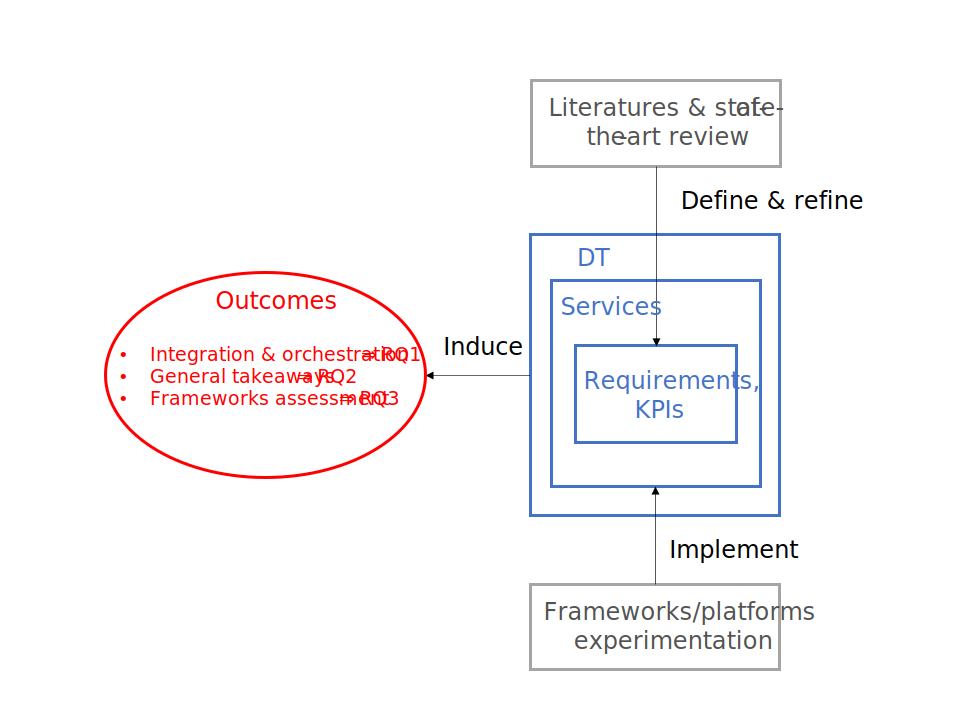
\includegraphics[scale=0.5]{figures/approach.pdf}
  \caption{Research approach}
  \label{fig:approach}
\end{figure}

\subsection{Project steps}\label{sec:prostep}
Section \ref{sec:approach} provides a holistic impression of how to approach the research. This section will continue to elaborate the exact steps to follow. We design a nine-step pathway to complete this project. The steps are divided to two phases, namely preparation phase, and implementation phase. The emphasis of the former phase is to conduct survey, and planning. The latter focuses on the software development to build the DT as well as to answer the research questions. Figure \ref{fig:researchsteps} shows the steps.

The reason we want to split the services to the `1+3' arrangement in step 4 is because we want to examine and compare all the proposed frameworks in the first place before committing to one. As a result, the prioritized service has to be simple to prototype within a short period. Furthermore, that service shall highlight the capabilities of each framework with respect to handling integration and orchestration.

Hereby we decide to choose `S1: production prediction' as our first service to implement. This decision is based on the two factors, simplicity and completeness, mentioned earlier. For the first factor, we realize S2 and S4 pose a higher threshold of technical effort in order to develop successfully. In S2, the requirements (see Section \ref{sec:reqkpis}) ask to handle the triggering of models and actuators promptly, while maintaining a stable calibration. This implies a great endeavor is required for tuning the actuators in order to adapt to different frameworks. Hence we will not use S2 as a rapid prototype in step 5. S4 follows a similar reasoning as its requirements require a flexible data ownership management, which is highly dependent on the sensors calibrations and significant adaptations under different frameworks. Although S3 is not as technical demanding as S2 and S4, however, semantically speaking, `what-if scenarios' is considered an extension to the `production prediction' service. Functionality-wise, S3 is based on many premises of S1 as well. Therefore, we think it is unnatural to implement S3 before S1. We argue that S1 is also qualifying in the completeness factor by looking at how each framework would utilize its features to fulfill S1 requirements and KPIs---detailed in Section \ref{sec:frameworks}.

 \begin{figure}[hbt!]
  \centering
  \includegraphics[scale=0.6]{figures/researchsteps.pdf}
  \caption{Project steps}
  \label{fig:researchsteps}
\end{figure}

\subsection{DT implementation workflow}\label{sec:5step}
During the implementation phase (project step 5 to 9), having setpoints helps us to judge whether the DT has met an acceptable level of development. One way of doing that is to check the corresponding requirements and KPIs of the services. From another angle, one can examine the DT by comparing it against a reference workflow to see what level it is at in term of complexity. Here we introduce a workflow which has been tailored for the bioprocessing theme.

Tao's 5D reference model introduced in Section \ref{sec:dtmodel} provides a glance of entities management in DTs. However, it does not address the varying maturities of the models in different attempts at developing a DT. For this purpose, Udugama et al. \cite{Udugama2021} propose a five-step workflow to implement a DT in bioprocessing. The workflow progresses in increasing order of mathematical complexity and functional requirements.

\begin{figure}[hbt!]
  \centering
  \includegraphics[scale=0.9]{figures/fivestep.pdf}
  \caption{The five-step implementation. This approach has been demonstrated in a design of DT for monoclonal antibodies manufacturing \cite{Helgers2022}}
  \label{fig:fivestep}
\end{figure}

\begin{enumerate}

  \item \textbf{Steady‑state model}: consisted of a mass and energy balance of the different key compounds in a reaction. These models are mathematical expressions of a process
that are not time-dependent and hence carry no accumulation
term.
  \item \textbf{Dynamic model}: contains time-based derivative terms on all variables of interest.
  \item \textbf{Validated model}: extends the capabilities of dynamic process models, such that it needs to be validated against process data obtained from an actual physical process.
  \item \textbf{Digital Shadow}: consistent with the definition given in Section \ref{sec:dt}; An one-way real-time monitoring model.
  \item \textbf{Digital Twin}: consistent with the definition given in Section \ref{sec:dt}; A two-way real-time monitoring and control model.
  
\end{enumerate}

As illustrated in Figure \ref{fig:fivestep}, the five-step view offers a systematic method in DT building, and a way to measure the maturity of a given DT. For the specific DT in this project, we aim for the `level 5' DT---a bidirectional model-based monitoring and control scheme---whenever applicable to the proposed services.

\pagebreak
\section{Preliminary outcomes}
Following the project steps proposed in Section \ref{sec:prostep}, we present the preliminary results for step 1, characteristic identifications in Section \ref{sec:char}; step 2,  requirements and KPI definitions in Section \ref{sec:reqkpis}; and step 3, frameworks comparison in Section \ref{sec:frameworks}.   

\subsection{Characteristics identifications}\label{sec:char}
Prior to deciding the key ingredients of integration and orchestration for certain services, it is helpful to firstly survey what characteristics are generally considered desirable across various use cases. These characteristics reoccur in the remarks which are found in the gathered studies. We classify them into either integration or orchestration based on the definitions given in Section \ref{sec:prodef}. Table \ref{tab:char} presents the found results.

\begin{table}[hbt!]
\centering
\begin{tabular}{|l|l||l|l|}
\hline
\textbf{Label} & \textbf{Integration}           & \textbf{Label} & \textbf{Orchestration}              \\ \hline
I1 & Configurability of parameters and time advancement & O1 & Control workflow and execution sequence \\ \hline
I2             & Automated code/data generation & O2             & Ontology checking                   \\ \hline
I3             & Data exchange consistency      & O3             & Managing mixed fidelity/granularity \\ \hline
I4             & Plug \& play modularity        &                &                                     \\ \hline
\end{tabular}
\caption{Identified characteristics}
\label{tab:char}
\end{table}

Statement I1 can be further broken down to two parts. First is the adjustability of initialization of the subsystems. As Tolksdorf et al. \cite{Tolksdorf2016} point out, upon the convergence of sub-models into one flowsheet, process engineers often face the challenge of guessing sensible initial values as the sub-models no longer are transparent to them, and a poor guess can easily lead to underperforming models. Therefore, it is argued that the accessibility to critical parameters throughout the whole process is essential to integration. The second part is related to the importance of multirate modeling with dynamic time management. In \cite{Neema2014}, the researchers experiment with varying execution step-sizes for a vehicle DT, showing that to a certain degree, distributed components---referred as federates---can be ran with different clocks rate and still produce matching results. The ability to parameterize time advancement extends flexibility in the platform under design.

I2 refers to the required automation upon combining models in order to reduce human errors. As chemical process optimizations are rarely accomplished by one single program, manually interfacing simulation packages from multiple vendors becomes impractical as soon as the system grows large \cite{Krone2020}. A systematic method to generate `glue codes' and data adaptation is an ideal solution. In practice, a hybrid scheme with varying levels of automation to trim down the hand-tuning effort is considered relevant in most cases.

I3 suggests in the case when a variable is transferred from one model to another, it shall retain its structure and its dependency relation with other objects. An important implication of this property occurs when several solvers are working on shared data. If information about algebraic dependencies between outputs and inputs are supplied, the importing tool is able to detect and handle algebraic loops automatically \cite{Blochwitz2011}.
 
The plug and play property in I4 implies not only the ease of use for the operator, but also the support for templates and instantiation. Actor-oriented design---also used in Ptolemy II---orthogonalizes component definition and component composition, allowing them to be considered independently \cite{Lee2004}. It promotes modularity which in turn reduces the associated design cost. 

\begin{figure}[hbt!]
  \centering
  \includegraphics[scale=1]{figures/o2ont.pdf}
  \caption{Errors that can be detected by ontology checking  \cite{Ptolemaeus2014}}
  \label{fig:o2ont}
\end{figure}

As described in the problem definition in Section \ref{sec:prodef}, O1 reinforces the importance of effective scheduling. One of the key factors that influences the workflow between models is coupling \cite{Karolius2018}, that is, how tightly are models intertwining with one another. A loose coupling relation generally requires less complex schedules. One may use strategies such as using an external framework to de-couple a pair of inherently coupled models. Other considerations, such as atomicity, might be required should there be concurrent processes.

Statement O2 discusses ontology, which is the explicit organization of constituent concepts and the relations between those concepts. More specifically, ontology can help to express the intended use of a model. In \cite{Ptolemaeus2014}, it is indicated that errors may arise from ontology inconsistencies, as illustrated in Figure \ref{fig:o2ont}.

In contrast to the emphasis on time step configurability in I1, O3 raises attention to the time synchronization and convergence across different models. For instance, merging discrete-time and continuous-time models by techniques of sampling and zero order hold; another example, signaling between time and untimed models. In the case of FMI, an event instant may be driven by a predefined time event or at the transition of state event indicators \cite{Blochwitz2011}. This is to allow numerical robustness, and is a part of the FMI feature which is known as `hybrid ODE'.

\subsection{Requirements and KPIs}\label{sec:reqkpis}
The requirements are defined such that they should entail the integration and orchestration characteristics found in Section \ref{sec:char}, in the meantime be tailored to the semantic goal of individual services. We must also keep in mind the 5D model of DTs, in which each requirement can be mapped to one or more connections between the other dimensions---namely VE, PE, service, and data---in the DT. 

In addition, several KPIs are set out to evaluate the effectiveness of the DT in terms of how it satisfies the requirements. In principle, each KPI should be a measurable metric that reflects a certain aspect of system performance or non-functional quality. The KPIs are defined in relation to the specific requirements they address. In other words, we develop the KPIs by analyzing the corresponding requirements and capture the measurable properties in them. Subsequently, we proceed to find a closely matching indicator, and use it as the measurement of those properties.   

\subsubsection{Production prediction}
In Table \ref{tab:s1rqkpi}, the top part shows the proposed requirements for S1, and the corresponding integration and orchestration (I \& O) implications they address to. The bottom part of the table shows the KPIs and their related requirements. R1 and R3 are associated to the VE-PE connection, whereas R2 relates to the parameterization of the VE-Service connection. Prior to the process startup, it is important to recognize exactly which parameters need to be configured and how often this is needed. Lastly, R4 represents the VE-Data connection.

\begin{table}[hbt!]
\centering
\begin{tabularx}{0.8\textwidth}{|p{1cm}|X|p{1.5cm}|}
\hline
\multicolumn{3}{|c|}{\textbf{Requirements}} \\
\hline
\textbf{Label} & \textbf{Requirement description} & \textbf{I \& O} \\ 
\hline            
R1 & The model state variables shall be validated with real-time empirical data. & I3, O2, O3 \\ 
\hline
R2 & The operator shall be able to configure the initial model parameters based on the given materials and resources. & I1 \\ 
\hline
R3 & The model parameters shall be automatically updated based on the latest real-time data. & I2, I3, O1 \\ 
\hline
R4 & The model may be interrogated for its past instances in order to optimize its present parameters. & I1, I4, O1 \\ 
\hline \hline
\end{tabularx}
\begin{tabularx}{0.8\textwidth}{|p{1cm}|p{2cm}|X|p{1.5cm}|}
\multicolumn{4}{|c|}{\textbf{KPIs}} \\ 
\hline
\textbf{Label} & \textbf{Indicator} & \textbf{Description} & \textbf{Relevance} \\ 
\hline
KPI1 & Rate of convergence & How fast the error of prediction against real-world data reaches an accepted lower threshold. & R1, R4 \\ 
\hline
KPI2 & Latency & How far is the model time behind real-world time. & R3 \\ 
\hline
KPI3 & Data availability & What is the amount of historical data that is useful in performing prediction. & R4 \\ 
\hline
KPI4 & Reconfigurability & How many parameters need to be set at startup time, and how many can be adjusted during runtime. & R2 \\ 
\hline
\end{tabularx}
\caption{S1 requirements and KPIs}
\label{tab:s1rqkpi}
\end{table}

\subsubsection{Production control}
Table \ref{tab:s2rqkpi} shows the requirements and KPIs for S2. It can be argued that R1 and R2 are complementary, as they represent the two way connection of VE-PE, which implies the condition of one trigger direction affect to that of another. The implication of R3 is that the model possess the contextual information of the physical process. In other words, the behavioral characteristics and information of the actuators are taken into account of the model computation, such that the transient behaviors can be kept to minimum. 

\begin{table}[hbt!]
\centering
\begin{tabularx}{0.8\textwidth}{|p{1cm}|X|p{1.5cm}|}
\hline
\multicolumn{3}{|c|}{\textbf{Requirements}} \\
\hline
\textbf{Label} & \textbf{Requirement description} & \textbf{I \& O} \\ 
\hline            
R1 & The model optimization may be triggered on the detected disturbance, time, or plant-wide performance. & O1, O2, O3 \\ 
\hline
R2 & The controller calibration may be triggered on time, or state variables deviation. & I2, O1, O2, O3 \\ 
\hline
R3 & The model shall ensure that the calibrations comply with the controller's desired operating range. & I1, O1, O2 \\ 
\hline \hline
\end{tabularx}
\begin{tabularx}{0.8\textwidth}{|p{1cm}|p{2cm}|X|p{1.5cm}|}
\multicolumn{4}{|c|}{\textbf{KPIs}} \\ 
\hline
\textbf{Label} & \textbf{Indicator} & \textbf{Description} & \textbf{Relevance} \\ 
\hline
KPI1 & Stableness of transitory behaviors & How long is the overshoots or undershoots period occurring before steady state. & R3 \\ 
\hline
KPI2 & System timeliness & What is the response time of triggering. & R1, R2 \\ 
\hline
\end{tabularx}
\caption{S2 requirements and KPIs}
\label{tab:s2rqkpi}
\end{table}

\subsubsection{What-if scenarios}
Table \ref{tab:s3rqkpi} shows the requirements and KPIs for S3. That being said, R1, R2, and R3 all address the VE-service connection. KPI3 highlights the human-in-the-loop idea mentioned in Section \ref{sec:dt}. As the end goal of what-if scenarios is to enable the operator to explore alternatives so they can gain a better assessment of the decisions and risks, delivering the scenarios to the operator smoothly becomes a crucial factor to the success of the operation.

\begin{table}[hbt!]
\centering
\begin{tabularx}{0.8\textwidth}{|p{1cm}|X|p{1.5cm}|}
\hline
\multicolumn{3}{|c|}{\textbf{Requirements}} \\
\hline
\textbf{Label} & \textbf{Requirement description} & \textbf{I \& O} \\ 
\hline            
R1 & The scenario-dependent data shall be stored and handled separately from the master data. & I4 \\ 
\hline
R2 & The scenarios shall be readily applied, reset, and removed without affecting the master schedule. & I1, I2, I4, O1 \\ 
\hline
R3 & The iterations of scenario may be managed under version control. & I2 \\ 
\hline \hline
\end{tabularx}
\begin{tabularx}{0.8\textwidth}{|p{1cm}|p{2cm}|X|p{1.5cm}|}
\multicolumn{4}{|c|}{\textbf{KPIs}} \\ 
\hline
\textbf{Label} & \textbf{Indicator} & \textbf{Description} & \textbf{Relevance} \\ 
\hline
KPI1 & Scalability & To what extent are the additional space and time bounded. & R1, R2, R3 \\ 
\hline
KPI2 & Accessibility & Are the model instances of the scenarios easily accessible to the operator. & R1, R3 \\ 
\hline
KPI3 & Modularity & Is changeover of the setup for each scenario easily adaptable. & R2 \\
\hline
\end{tabularx}
\caption{S3 requirements and KPIs}
\label{tab:s3rqkpi}
\end{table}

\subsubsection{Predictive maintenance}
Table \ref{tab:s4rqkpi} shows the requirements and KPIs for S4. We argue R1 and R2 represent the VE-PE connection. R3 accounts for the chained connection of VE-PE-Data. The term data ownership in R3 refers to the participation in the generation, processing, value addition or analysis of data \cite{Rasheed2020}. In DTs this can be complicated as there is a great diversity of involving parts across physical to virtual space. Data ownership management consists mainly of three actions: engaging, disengaging, and transferring. A smooth transition between these actions is regarded crucial especially for data-driven predictive models.

\begin{table}[hbt!]
\centering
\begin{tabularx}{0.8\textwidth}{|p{1cm}|X|p{1.5cm}|}
\hline
\multicolumn{3}{|c|}{\textbf{Requirements}} \\
\hline
\textbf{Label} & \textbf{Requirement description} & \textbf{I \& O} \\ 
\hline            
R1 & Dynamic data acquisition shall used to update the static attributes in the predictive model & I2, I3, O1, O2, O3 \\ 
\hline
R2 & Real-time measurements and simulated results shall be used in the retrofitting of the predictive model  & I1, I2, O1, O2, \\ 
\hline
R3 & Data ownership shall have high degree of flexibility and be transferable within the DT in order to perform efficient data prepossessing & I2, I3, O3 \\ 
\hline \hline
\end{tabularx}
\begin{tabularx}{0.8\textwidth}{|p{1cm}|p{2cm}|X|p{1.5cm}|}
\multicolumn{4}{|c|}{\textbf{KPIs}} \\ 
\hline
\textbf{Label} & \textbf{Indicator} & \textbf{Description} & \textbf{Relevance} \\ 
\hline
KPI1 & Accuracy & What is the error of the predictive model against real-world measurement & R1, R2\\ 
\hline
KPI2 & Impact of missing data & How missing data may affect the overall performance of predictive model & R1, R2 \\ 
\hline
KPI3 & Data quality & How much volume, variety, and veracity of the data is lost as the result of transferring and fusion & R3 \\
\hline
\end{tabularx}
\caption{S4 requirements and KPIs}
\label{tab:s4rqkpi}
\end{table}


\subsection{Frameworks comparison}\label{sec:frameworks}
We have mentioned actor-orientated architecture---adopted by Ptolemy II---and SOA used as the approaches for orchestration in Section \ref{sec:orctool}. In this section, we proceed to investigate the possibility of adopting them as development framework for the microbrewery DT. The key selection criteria for deciding a development framework are that the development environment should support the proposed requirements for the services. Firstly, an emerging methodology known as TwinOps will be introduced. Secondly, we will describe a flavor of frameworks based on SOA, called LwM2M network. After that, Ptolemy II will be reviewed once again, this time with extra attention given to the modeling infrastructure provided by it.

\begin{figure}[hbt!]
  \centering
  \includegraphics[scale=0.6]{figures/devops.pdf}
  \caption{DevOps concept portrayed by the infinite loop}
  \label{fig:devops}
\end{figure}

\begin{figure}[hbt!]
  \centering
  \includegraphics[scale=1]{figures/twinopsloop.pdf}
  \caption{TwinOps forward and feedback loop \cite{Hugues2020}}
  \label{fig:twinopsloop}
\end{figure}

Proposed by Hugues et al. \cite{Hugues2020}, TwinOps borrows the concept of DevOps \cite{Ebert2016} from software engineering, where the development and operation are merged into one continuous loop of forward delivery and feedback (see Figure \ref{fig:devops}). In TwinOps, the `Dev' part transcends to DT models integration and target codes generation; and the `Ops' part is overloaded with data collection and analysis in DTs. As illustrated in Figure \ref{fig:twinopsloop}, the black arrows are the code generation forwarded to various targets, and the orange arrows represented the data analytic feedback. In the work of Hugues, the exemplified case study of a monitoring system for a building utilizes the technology stack consisting of AADL, LNT, C, FMI, and Azure to build a pipeline. The AADL toolchain is responsible for specifying the modeling architecture as well as requirements. The LNT target enables model-checking. The C/FMI target supports modeling and simulation of the virtual entity. Finally the C/Azure target leverages containerized cloud system to deploy execution command on the physical entity.

\begin{figure}[hbt!]
  \centering
  \includegraphics[scale=0.6]{figures/lwm2m.pdf}
  \caption{LwM2M deployment \cite{oma2019}}
  \label{fig:lwm2m}
\end{figure}

M2M---short for machine-to-machine---network is a popular topic in IoT applications. One of the open source frameworks is called LightweightM2M (LwM2M) which is created by the Open Mobile Alliance (OMA) with the emphasis on efficient bandwidth \cite{oma2020}. It is essentially a protocol stack that supports various operations from bootstrapping and registration, to device and service management within sensor networks. Figure \ref{fig:lwm2m} illustrates the overall deployment view of the LwM2M architecture. When applied to DT construction, one can map the physical entities to LwM2M client objects, and the virtual entities to LwM2M server objects. The idea is to leverage the protocol to perform the necessary integration and orchestration. 

\begin{figure}[hbt!]
  \centering
  \includegraphics[scale=0.8]{figures/pt2meta.pdf}
  \caption{Meta model of Ptolemy II}
  \label{fig:pt2meta}
\end{figure}

In \cite{Ptolemaeus2014} it presents a meta model that describes the abstract syntax of Ptolemy II software architecture, as seen in Figure \ref{fig:pt2meta}. Every component in a Ptolemy II model is an instance of the \texttt{NamedObj} class. There are four subclasses of \texttt{NamedObj}. These are called \texttt{Attribute}, \texttt{Entity}, \texttt{Port}, and \texttt{Relation}. The \texttt{Relation} class represents communication path between entities. The \texttt{Port} class has links to \texttt{Relation}, and it also hosts the \texttt{Receiver} interface that implements methods relating to data transmitting. Together they can be used to manage the model integration in DTs. On the other hand, for orchestration, it can be achieved in the \texttt{Executable} interface which is implemented by \texttt{Director}. The interface coordinates the iterations among actors based on the rules of the selected MoC.

\begin{table}[]
\centering
\begin{tabular}{|l|l|llll|lll|lll|lll|}
\hline
 &
   &
  \multicolumn{4}{c|}{\textbf{S1}} &
  \multicolumn{3}{c|}{\textbf{S2}} &
  \multicolumn{3}{c|}{\textbf{S3}} &
  \multicolumn{3}{c|}{\textbf{S4}} \\ \hline
 &
  \textbf{Strength} &
  \multicolumn{1}{l|}{R1} &
  \multicolumn{1}{l|}{R2} &
  \multicolumn{1}{l|}{R3} &
  R4 &
  \multicolumn{1}{l|}{R1} &
  \multicolumn{1}{l|}{R2} &
  R3 &
  \multicolumn{1}{l|}{R1} &
  \multicolumn{1}{l|}{R2} &
  R3 &
  \multicolumn{1}{l|}{R1} &
  \multicolumn{1}{l|}{R2} &
  R3 \\ \hline
\multirow{3}{*}{\textbf{TwinOps}} &
  Bridging Dev and Ops &
  \multicolumn{1}{l|}{} &
  \multicolumn{1}{l|}{} &
  \multicolumn{1}{l|}{} &
  O &
  \multicolumn{1}{l|}{O} &
  \multicolumn{1}{l|}{O} &
  O &
  \multicolumn{1}{l|}{} &
  \multicolumn{1}{l|}{} &
   &
  \multicolumn{1}{l|}{O} &
  \multicolumn{1}{l|}{} &
  O \\ \cline{2-15} 
 &
  Multiple targets code generation &
  \multicolumn{1}{l|}{} &
  \multicolumn{1}{l|}{O} &
  \multicolumn{1}{l|}{} &
   &
  \multicolumn{1}{l|}{} &
  \multicolumn{1}{l|}{} &
   &
  \multicolumn{1}{l|}{O} &
  \multicolumn{1}{l|}{O} &
   &
  \multicolumn{1}{l|}{} &
  \multicolumn{1}{l|}{} &
   \\ \cline{2-15} 
 &
  Traceable activities via containerization &
  \multicolumn{1}{l|}{} &
  \multicolumn{1}{l|}{} &
  \multicolumn{1}{l|}{} &
   &
  \multicolumn{1}{l|}{} &
  \multicolumn{1}{l|}{} &
   &
  \multicolumn{1}{l|}{} &
  \multicolumn{1}{l|}{O} &
  O &
  \multicolumn{1}{l|}{} &
  \multicolumn{1}{l|}{O} &
   \\ \hline
\multirow{3}{*}{\textbf{LwM2M}} &
  Bootstrapping and registration &
  \multicolumn{1}{l|}{} &
  \multicolumn{1}{l|}{O} &
  \multicolumn{1}{l|}{} &
  O &
  \multicolumn{1}{l|}{} &
  \multicolumn{1}{l|}{} &
   &
  \multicolumn{1}{l|}{} &
  \multicolumn{1}{l|}{} &
  O &
  \multicolumn{1}{l|}{} &
  \multicolumn{1}{l|}{} &
   \\ \cline{2-15} 
 &
  Data communication &
  \multicolumn{1}{l|}{O} &
  \multicolumn{1}{l|}{} &
  \multicolumn{1}{l|}{O} &
   &
  \multicolumn{1}{l|}{O} &
  \multicolumn{1}{l|}{O} &
  O &
  \multicolumn{1}{l|}{} &
  \multicolumn{1}{l|}{} &
   &
  \multicolumn{1}{l|}{O} &
  \multicolumn{1}{l|}{} &
   \\ \cline{2-15} 
 &
  Objects and resource management &
  \multicolumn{1}{l|}{} &
  \multicolumn{1}{l|}{} &
  \multicolumn{1}{l|}{} &
   &
  \multicolumn{1}{l|}{O} &
  \multicolumn{1}{l|}{O} &
   &
  \multicolumn{1}{l|}{} &
  \multicolumn{1}{l|}{} &
   &
  \multicolumn{1}{l|}{} &
  \multicolumn{1}{l|}{} &
  O \\ \hline
\multirow{3}{*}{\textbf{Ptolemy II}} &
  Pre-defined MoC &
  \multicolumn{1}{l|}{O} &
  \multicolumn{1}{l|}{} &
  \multicolumn{1}{l|}{} &
   &
  \multicolumn{1}{l|}{} &
  \multicolumn{1}{l|}{} &
   &
  \multicolumn{1}{l|}{} &
  \multicolumn{1}{l|}{} &
   &
  \multicolumn{1}{l|}{O} &
  \multicolumn{1}{l|}{} &
   \\ \cline{2-15} 
 &
  Support for time model &
  \multicolumn{1}{l|}{O} &
  \multicolumn{1}{l|}{} &
  \multicolumn{1}{l|}{} &
   &
  \multicolumn{1}{l|}{O} &
  \multicolumn{1}{l|}{O} &
   &
  \multicolumn{1}{l|}{} &
  \multicolumn{1}{l|}{} &
   &
  \multicolumn{1}{l|}{O} &
  \multicolumn{1}{l|}{} &
   \\ \cline{2-15} 
 &
  Actor-orientated modelling &
  \multicolumn{1}{l|}{} &
  \multicolumn{1}{l|}{} &
  \multicolumn{1}{l|}{} &
   &
  \multicolumn{1}{l|}{} &
  \multicolumn{1}{l|}{} &
  O &
  \multicolumn{1}{l|}{} &
  \multicolumn{1}{l|}{} &
   &
  \multicolumn{1}{l|}{} &
  \multicolumn{1}{l|}{} &
   \\ \hline
\end{tabular}
\caption{Development framework comparison}
\label{tab:dfcomp}
\end{table}

In summary, shown in Table \ref{tab:dfcomp} is a tentative assessment of each framework choice that has been introduced so far. In the table, we examine what service requirements could be benefited from the respective framework's strengths. Besides the inherent strengths of the framework's features, it is also necessary to discuss about the practicality side of developing with these frameworks. Here we recognize some deficiencies that might occur during the implementation phase. Remedies to mitigate the deficiencies will also be proposed.

The first deficiency is the ability to capture the high-level relationship of the DT dimensions, and to ensure its semantic soundness. In Ptolemy II it is enabled by its self-explanatory graphical modeling environment, along with some limited capability of model error checking. In an use case of TwinOps, SysML is adopted for describing the models architecture. Further, it leverages on AADL to refine the more detailed component parts. In LwM2M there is no specified way of achieving model description. One solution can be using MBSE instruments such as SysML or UML to support preliminary analysis.

Another deficiency we predict that might occur in one or more of the frameworks is related to the methods of schedulability analysis and implementing schedules. In Ptolemy II there are built-in MoCs and sophisticated receiver queues, for instance, FIFO or LIFO implementations, that are able to support this aspect. In TwinOps it utilize the FMI approach, such that the master algorithm is made in AADL, which then be used to orchestrate the FMUs. LwM2M has described a (layered-)control scheme and the option to place objects in logical group in its protocol specification. The approaches in these frameworks are all considered valid, although they can be further enhanced by using sequence diagram and data flow diagram to formalize the control and data flow respectively.

The third deficiency is concerned with data communication pattern. Ptolemy II has predefined `relation' and `port' object to handle it, however, a potential shortcoming is that entities must be transformed to actors in order to work compatibly. In TwinOps, the detailed connection paths are modeled in AADL, then the pipeline will generate containerized binaries to specific targets. In LwM2M one can adopt various common common IoT strategies such as client/server (e.g., HTTP), pub/sub (e.g., MQTT) to achieve data communication. For the DT domain, it is advisable to highlight on the automation and scaling aspects.

The fourth deficiency relates to artifacts management such as data storage. In Ptolemy II there are few remarks about logging. TwinOps describes the usage of Azure IoT platform \cite{azureiot} for the distribution of containers. In LwM2M it is not specified, but cloud database servers are known to be advantageous in various M2M applications \cite{Verma2016}. Building an offline or cloud database system is a sound approach, nevertheless in the DT context automation of version control is considered one of the focuses. 

\pagebreak
\section{Project planning}
In this section we propose a roadmap for this research project. The implementation phase is divided into two stages, just as shown in the project steps. In the first stage, a service---in this case, production prediction---from the four available DT services will be selected and implemented with the three frameworks outlined in Section \ref{sec:frameworks}. This is due to completion in mid-June. After that, an analysis with respect to integration and orchestration will be made. For the second stage, we will decide the most suitable framework out of three based on the previous experimentation and comparison, thus implementing the other three services with that framework. The expected completion date for the second stage is mid-August. All implementations will be tested throughout the project. The proposed timeline is presented in Figure \ref{fig:timeline}.

\begin{figure}[hbt!]
  \centering
  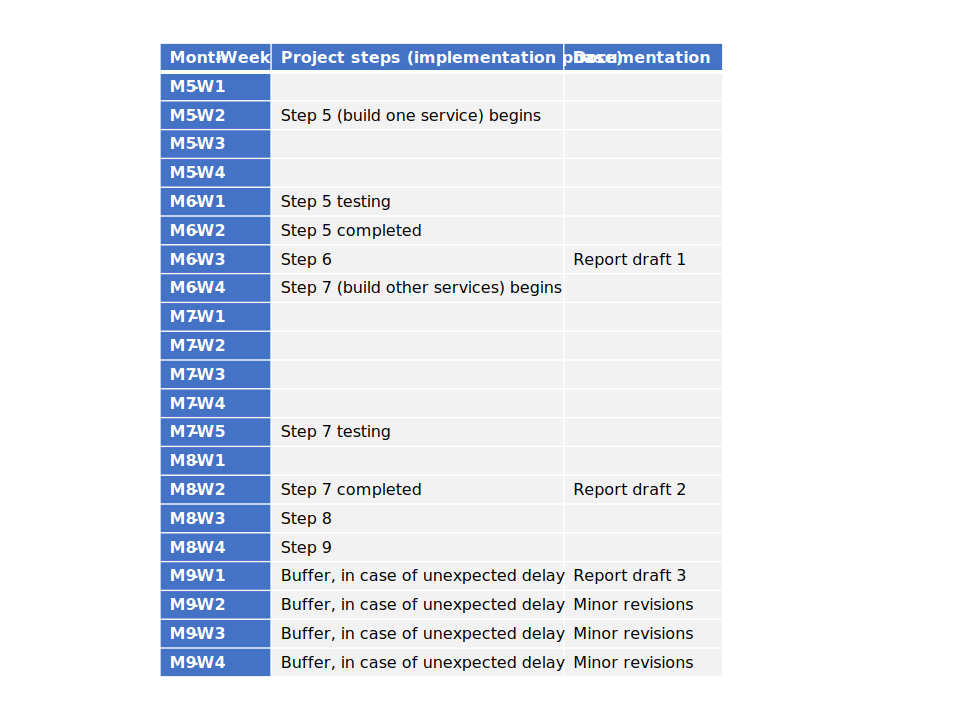
\includegraphics[scale=0.8]{figures/timeline.pdf}
  \caption{Project timeline}
  \label{fig:timeline}
\end{figure}

\pagebreak
\bibliographystyle{IEEEtran}
\bibliography{IEEEabrv,literature}

\end{document}
